\chapter{植物营养发育：分生组织与生长}\label{ch:b2:plant-meristems}

一棵在大教堂落成时还是幼苗的橡树，至今
仍每年增加一圈\omterm{def:b2:plant-meristems:wood}{木材}，仍在每个春天长出新叶，
仍把新的根尖推进土壤。没有哪种动物
能做到这一点；马四岁便停止生长。两者的区别在于
植物在每个茎的顶端、每条根的根尖，以及
每根树干内部的薄圆柱层中，始终保留着若干小群胚性细胞，
——即\emph{\omterm{def:b2:plant-meristems:meristem}{分生组织}}——它们永不停止分裂，
并只要植物存活，就不断向外、向上构建植物体。本章
讨论两类顶端\omterm{def:b2:plant-meristems:meristem}{分生组织}如何组织并受到调控，
植物细胞如何生长，激素如何决定
茎的形态，以及树干如何加粗。

\section{分生组织}

\begin{definition}[分生组织与两类生长]\label{def:b2:plant-meristems:meristem}
\index{分生组织}\index{茎尖分生组织}\index{根尖分生组织}\index{形成层}
\emph{分生组织}是一群小型、未\omterm{def:b2:cell-differentiation:differentiation}{分化}的
分裂细胞，在植物的整个生命周期中持续存在，并且
其全部组织都由其派生。\emph{茎尖分生组织}（SAM）
位于每个茎的顶端，产生叶、茎，并在适当季节产生花；
\emph{根尖分生组织}（RAM）位于每个根尖之后，产生
根；二者共同驱动\emph{初生生长}，即植物的
纵向伸长。\emph{侧生分生组织}——即\emph{\omterm{def:b2:plant-meristems:wood}{维管
形成层}}与\emph{木栓形成层}，二者均为位于茎和根内部的薄圆柱体——
驱动\emph{次生生长}，即使植物增粗的过程，
形成\omterm{def:b2:plant-meristems:wood}{木材}与\omterm{def:b2:plant-meristems:wood}{树皮}。植物的生长因此是\emph{无限生长的}：
分生组织可无限期持续下去，植物因而是一种模块化的
生物体，不断重复“叶–节–节间–芽”这一单元，只要
条件允许。每个腋芽都是一个\omterm{def:b2:angiosperm-reproduction:seed}{休眠}的 SAM，因此一株植物
携带数千个备用生长点。
\end{definition}

\begin{proposition}[茎尖]\label{prop:b2:plant-meristems:sam}
\index{叶序}\index{叶原基}\index{叶间隔期}
SAM 是一个直径约十分之一毫米的圆顶，由几百个
细胞构成。其外侧一到两层（\emph{原套}）只沿
表面的平行方向分裂，并形成表皮；其下方的团块
（\emph{原体}）则在所有平面上分裂。顶部有一个
\emph{中央区}，由缓慢分裂的\omterm{def:b2:cell-differentiation:differentiation}{干细胞}组成，为
\emph{周边区}提供分裂较快的细胞，其中\emph{\omterm{prop:b2:plant-meristems:sam}{叶
原基}}以规则的时间间隔形成凸起（即
\emph{\omterm{prop:b2:plant-meristems:sam}{叶间隔期}}，历时数小时至数天），并以规则的角度环绕
圆顶排列（即\emph{\omterm{prop:b2:plant-meristems:sam}{叶序}}：对生、轮生或螺旋状，按
\qty{137.5}{\degree}的黄金角排列，使每片新叶位于
其他叶留下的最大空隙中）。下方的\emph{肋区}
形成髓并使茎伸长。\omterm{prop:b2:plant-meristems:sam}{叶原基}形成于
\omterm{prop:b2:plant-meristems:apical}{生长素}积累于表层的部位，原基生长时
从周围吸取\omterm{prop:b2:plant-meristems:apical}{生长素}，这正是下一个原基尽可能远离它的原因：
该格局是
自组织的。
\end{proposition}

\begin{omfigure}
\begin{tikzpicture}[every node/.style={font=\scriptsize}]
  % dome
  \draw[thick, fill=omExo!12] (-2.2,0) .. controls (-2.2,1.6) and (-0.8,2.6) .. (0,2.6) .. controls (0.8,2.6) and (2.2,1.6) .. (2.2,0) -- (2.2,-1.4) -- (-2.2,-1.4) -- cycle;
  % tunica layers
  \draw[thick, omDef] (-2.2,0) .. controls (-2.2,1.5) and (-0.8,2.45) .. (0,2.45) .. controls (0.8,2.45) and (2.2,1.5) .. (2.2,0);
  \draw[thick, omDef] (-2.05,0) .. controls (-2.05,1.35) and (-0.75,2.3) .. (0,2.3) .. controls (0.75,2.3) and (2.05,1.35) .. (2.05,0);
  % zones
  \draw[thick, dashed, omThm, fill=omThm!15] (0,1.75) ellipse (0.6 and 0.55);
  \draw[thick, dashed, omProp] (0,0.9) ellipse (1.6 and 1.35);
  \draw[thick, dashed, omExo!70!black] (-0.9,-0.9) rectangle (0.9,-0.1);
  % primordia
  \draw[thick, fill=omExo!40] (-2.2,0.4) .. controls (-2.5,1.4) and (-1.6,1.9) .. (-1.55,1.3) .. controls (-1.5,0.9) and (-1.9,0.6) .. (-2.2,0.4);
  \draw[thick, fill=omExo!40] (2.2,0.2) .. controls (2.7,1.0) and (2.1,1.5) .. (1.75,1.1) .. controls (1.6,0.8) and (1.9,0.5) .. (2.2,0.2);
  % labels
  \draw (0.4,2.1) -- (3.2,2.6) node[right, align=left] {中央区：\\缓慢分裂的干细胞};
  \draw (1.3,0.5) -- (3.2,1.4) node[right, align=left] {周边区：\\快速分裂，叶原基};
  \draw (0.6,-0.5) -- (3.2,0.0) node[right, align=left] {肋区：髓，\\茎伸长};
  \draw (-1.7,1.5) -- (-3.0,2.4) node[left, align=right] {叶 \\原基};
  \draw (-1.2,2.05) -- (-3.0,1.2) node[left, align=right] {原套：仅表面 \\分裂};
  \draw (2.2,0.7) -- (3.2,-1.0) node[right, align=left] {下一个原基，\\按\qty{137.5}{\degree}旋转};
\end{tikzpicture}

{\small \omterm{def:b2:plant-meristems:meristem}{茎尖分生组织}纵切面：由一到两层表层细胞构成的原套，
覆盖在原体之上，顶部为\omterm{def:b2:cell-differentiation:differentiation}{干细胞}组成的中央区，
周边区中\omterm{prop:b2:plant-meristems:sam}{叶原基}向外凸起，以及
下方的肋区。}
\end{omfigure}

\begin{omfigure}
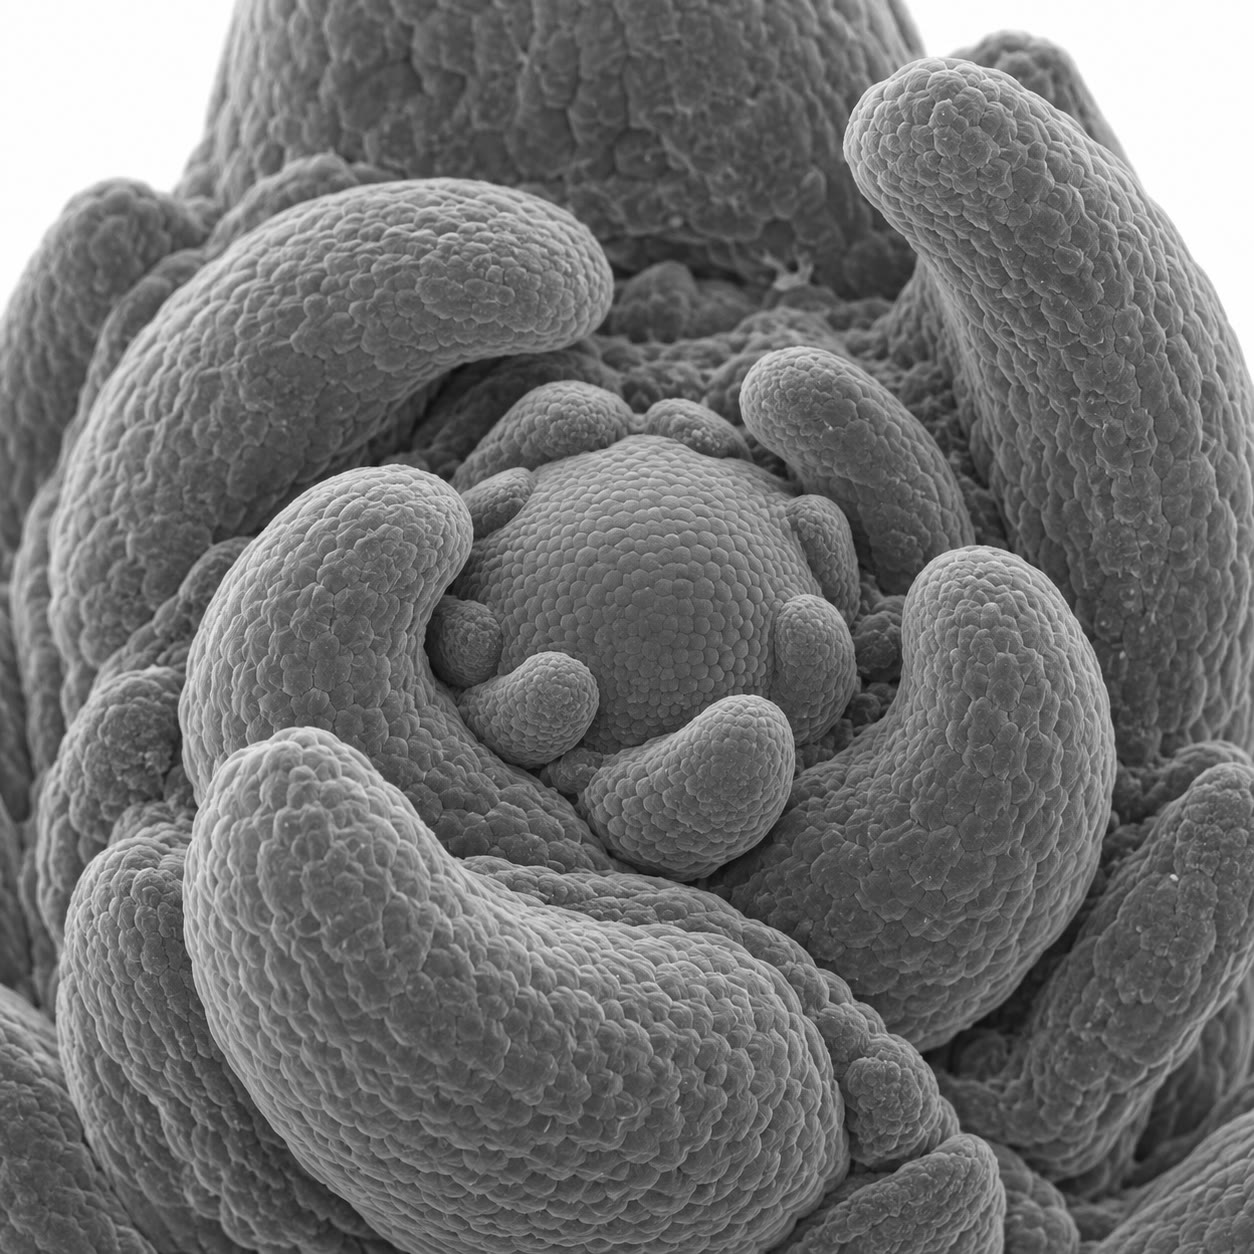
\includegraphics[width=0.44\linewidth]{images/book4/ai/b4-13-shoot-apex-sem.jpg}

{\small 扫描电子显微镜下的茎尖：
光滑的\omterm{def:b2:plant-meristems:meristem}{分生组织}圆顶，以及周围螺旋排列的\omterm{prop:b2:plant-meristems:sam}{叶原基}，
每个新原基都位于最宽的空隙中。}
\end{omfigure}

\begin{proposition}[维持干细胞：反馈回路]\label{prop:b2:plant-meristems:wus}
\index{WUSCHEL}\index{CLAVATA}\index{负反馈!分生组织}
\omterm{def:b2:cell-differentiation:differentiation}{干细胞}池的大小由一个回路维持恒定，该回路位于
两个基因之间。中央区正下方的细胞表达\omterm{prop:b2:cell-differentiation:transcriptional}{转录因子}
\emph{\omterm{prop:b2:plant-meristems:wus}{WUSCHEL}}（WUS），其产物向上迁移
进入上覆细胞，使其保持为\omterm{def:b2:cell-differentiation:differentiation}{干细胞}；\omterm{def:b2:cell-differentiation:differentiation}{干细胞}
又分泌一种小肽\emph{CLAVATA3}（CLV3），该肽
向下扩散，与表达 WUS 的细胞中的受体激酶（CLV1）结合，
并抑制 WUS。\omterm{def:b2:cell-differentiation:differentiation}{干细胞}越多，CLV3 越多，WUS 越少，
\omterm{def:b2:cell-differentiation:differentiation}{干细胞}随之减少；\omterm{def:b2:cell-differentiation:differentiation}{干细胞}越少，CLV3 越少，WUS 越多，
\omterm{def:b2:cell-differentiation:differentiation}{干细胞}随之增多。因此\omterm{def:b2:cell-differentiation:differentiation}{干细胞}池是一个受调控的量，
与\cref{ch:b2:reproductive-hormones}中的促性腺激素一样，
同一逻辑——来自受调控细胞群的信号抑制产生它的
因子——同样适用于根\omterm{def:b2:plant-meristems:meristem}{分生组织}。
\end{proposition}
\begin{proof}[证据]
Arabidopsis \emph{clavata} \omterm{def:b2:genome-diversification:mutation}{突变}体（克拉克、迈耶罗维茨，1990 年代）的
\omterm{def:b2:plant-meristems:meristem}{分生组织}膨大至正常大小的数倍，并多出
叶片、额外的花器官，以及扁化（扁平、带状）的
茎：制动机制已失效。\emph{wuschel} \omterm{def:b2:genome-diversification:mutation}{突变}体形成的\omterm{def:b2:plant-meristems:meristem}{分生组织}
在长出数片叶后停止，随后又形成新的\omterm{def:b2:plant-meristems:meristem}{分生组织}，每一个
又依次停止：加速机制已失效。双\omterm{def:b2:genome-diversification:mutation}{突变}体中
\emph{wuschel} \omterm{def:b2:meiosis-heredity:vocabulary}{表型}占优，表明 WUS 位于 CLV 下游；
将 CLV3 肽施于野生型茎尖，可在
数小时内抑制 WUS。
\end{proof}

\begin{proposition}[根尖]\label{prop:b2:plant-meristems:ram}
\index{根冠}\index{静止中心}\index{伸长区}\index{根毛}
根从位于\emph{\omterm{prop:b2:plant-meristems:ram}{根冠}}之后、受其保护的\omterm{def:b2:plant-meristems:meristem}{分生组织}中生长，
\omterm{prop:b2:plant-meristems:ram}{根冠}细胞在根尖穿过土壤时脱落，
并分泌润滑的黏液，还能感知重力（依靠
细胞内沉降的淀粉粒）。\omterm{def:b2:plant-meristems:meristem}{分生组织}中央有
由数百个细胞组成的\emph{\omterm{prop:b2:plant-meristems:ram}{静止中心}}，细胞很少分裂；
它使周围的原始细胞——\omterm{prop:b2:plant-meristems:ram}{根冠}、表皮、皮层和
维管柱的起始细胞——保持为\omterm{def:b2:cell-differentiation:differentiation}{干细胞}，其作用与 WUS
维持茎尖\omterm{def:b2:cell-differentiation:differentiation}{干细胞}相似。\omterm{def:b2:plant-meristems:meristem}{分生组织}之后是\emph{\omterm{prop:b2:plant-meristems:ram}{伸长
区}}，长约数毫米，细胞在此伸长十至
二十倍，推动根尖前进；随后是\emph{\omterm{def:b2:cell-differentiation:differentiation}{分化}
区}，表皮在此长出\emph{\omterm{prop:b2:plant-meristems:ram}{根毛}}，木质部和
韧皮部逐渐成熟。侧根并非起源于根尖，而是
起源于成熟根内部、木质部极点对侧的中柱鞘，
并穿过皮层向外伸出。\omterm{prop:b2:plant-meristems:apical}{生长素}在茎中合成后
向下运输，在根尖积累，统领整个结构；
\omterm{prop:b2:plant-meristems:ram}{静止中心}处的\omterm{prop:b2:plant-meristems:apical}{生长素}浓度最高。
\end{proposition}

\begin{omfigure}
\begin{tikzpicture}[every node/.style={font=\scriptsize}]
  % root outline
  \draw[thick, fill=omExo!10] (-1.0,4.5) -- (-1.0,0.6) .. controls (-1.0,-0.4) and (1.0,-0.4) .. (1.0,0.6) -- (1.0,4.5);
  % root cap
  \draw[thick, fill=omExo!45] (-0.9,0.8) .. controls (-1.1,-0.1) and (1.1,-0.1) .. (0.9,0.8) .. controls (0.5,0.4) and (-0.5,0.4) .. (-0.9,0.8);
  % meristem
  \fill[omThm!25] (-0.85,0.8) rectangle (0.85,1.7);
  \fill[omThm!70] (0,0.95) ellipse (0.25 and 0.12);
  % elongation zone
  \fill[omProp!20] (-0.85,1.7) rectangle (0.85,3.0);
  % differentiation zone with root hairs and vascular strand
  \fill[omDef!15] (-0.85,3.0) rectangle (0.85,4.5);
  \fill[omDef!50] (-0.15,3.0) rectangle (0.15,4.5);
  \foreach \y in {3.2,3.5,3.8,4.1,4.4} { \draw[omDef!80!black] (1.0,\y) -- (1.7,\y+0.1); \draw[omDef!80!black] (-1.0,\y) -- (-1.7,\y+0.1); }
  % lateral root primordium
  \draw[thick, fill=omThm!30] (0.15,4.0) .. controls (0.5,3.9) and (0.8,4.1) .. (0.9,4.3) .. controls (0.7,4.35) and (0.4,4.3) .. (0.15,4.3);
  % labels
  \draw (0.5,0.4) -- (2.2,0.2) node[right] {根冠};
  \draw (0.25,0.95) -- (2.2,0.9) node[right] {静止中心};
  \draw (0.85,1.4) -- (2.2,1.5) node[right] {分生组织（分裂）};
  \draw (0.85,2.4) -- (2.2,2.3) node[right, align=left] {伸长区：\\细胞伸长 $10\times$};
  \draw (1.5,3.6) -- (2.2,3.4) node[right] {根毛};
  \draw (0.0,4.2) -- (2.2,4.2) node[right] {维管柱};
  \draw (0.7,4.3) -- (2.2,4.9) node[right, align=left] {侧根原基 \\（源自中柱鞘）};
  \draw[->, thick] (-2.4,4.5) -- (-2.4,0.6); \node[left, rotate=90, anchor=south] at (-2.5,2.5) {生长素流向根尖};
\end{tikzpicture}

{\small 根尖：\omterm{prop:b2:plant-meristems:ram}{根冠}、带\omterm{prop:b2:plant-meristems:ram}{静止中心}的\omterm{def:b2:plant-meristems:meristem}{分生组织}，
\omterm{prop:b2:plant-meristems:ram}{伸长区}，以及带\omterm{prop:b2:plant-meristems:ram}{根毛}的\omterm{def:b2:cell-differentiation:differentiation}{分化}区，
其中有成熟导管。侧根从内部的中柱鞘开始发生。}
\end{omfigure}

\begin{omfigure}
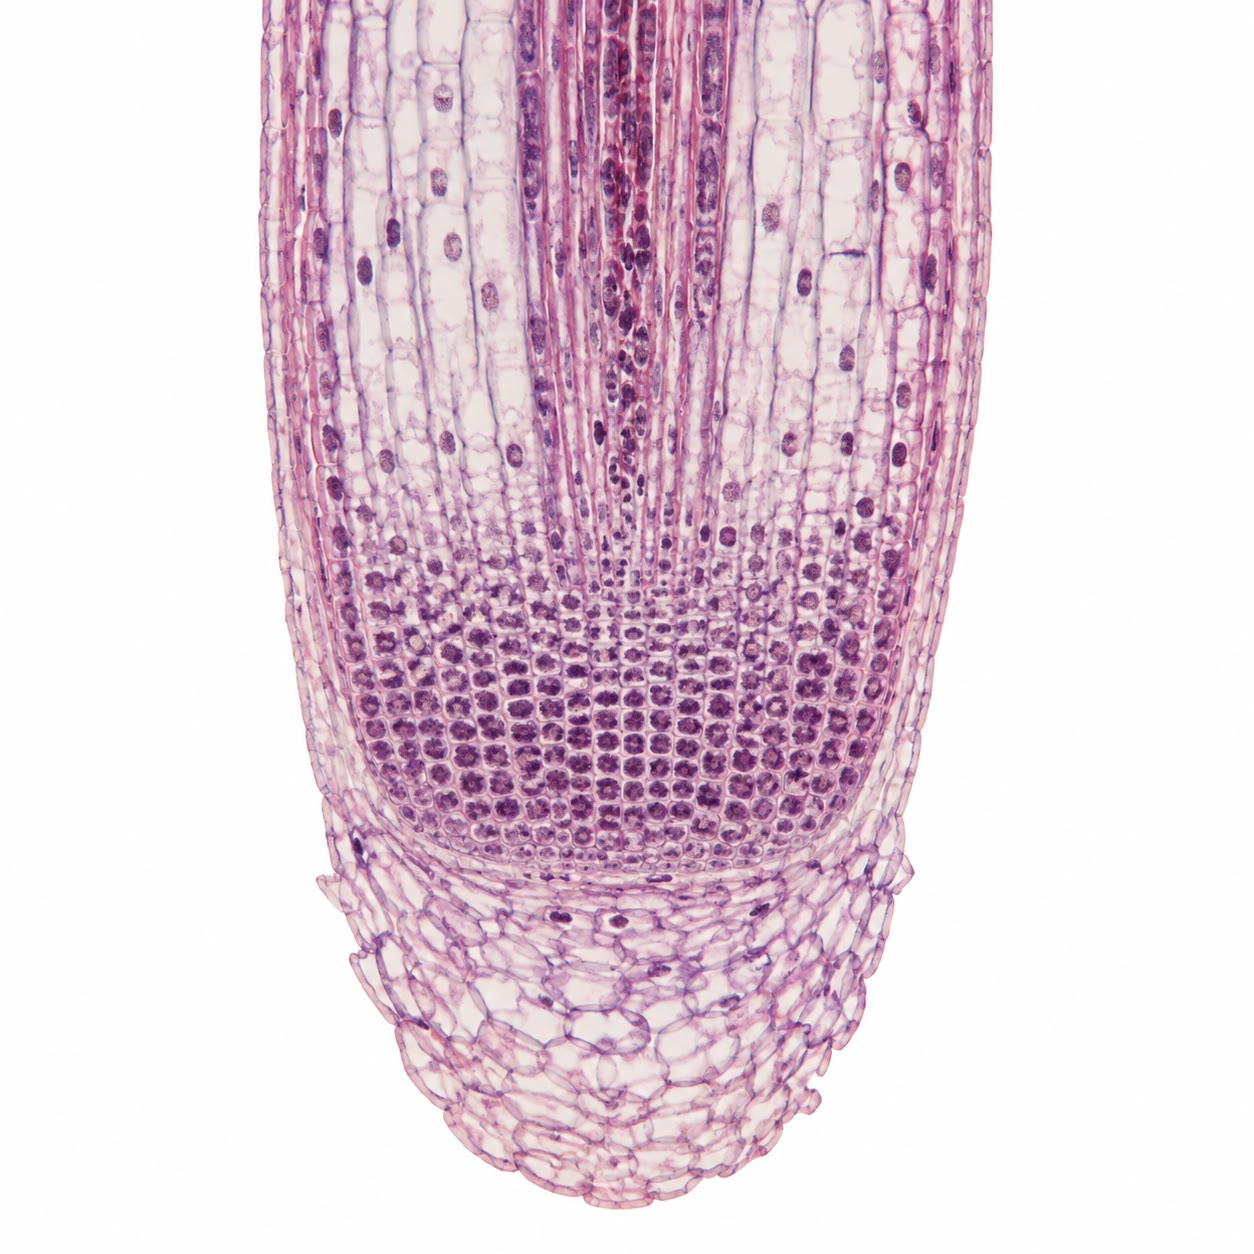
\includegraphics[width=0.42\linewidth]{images/book4/ai/b4-13-root-tip.jpg}

{\small 根尖纵切面：\omterm{prop:b2:plant-meristems:ram}{根冠}中疏松的细胞，
致密的\omterm{def:b2:plant-meristems:meristem}{分生组织}及其深色的细胞核，
以及上方正在伸长的细胞。}
\end{omfigure}

\section{植物细胞如何生长}

\begin{theorem}[洛克哈特方程]\label{thm:b2:plant-meristems:lockhart}
\index{膨压}\index{细胞壁!延展性}\index{洛克哈特方程}
植物细胞靠其自身内容物施加的压力拉伸\omterm{def:b2:unicellular-diversity:prokaryote}{细胞壁}而生长。
\omterm{def:b2:unicellular-diversity:prokaryote}{细胞壁}只有在膨压超过阈值
$Y$ 时才不可逆地形变，且速率与超出量成正比：
长度为 $L$ 的细胞，其相对生长速率为
\[
\frac{1}{L}\frac{\mathrm{d}L}{\mathrm{d}t} = \phi\,(P - Y) \quad (P > Y),
\]
其中 $P$ 为膨压，$\phi$ 为\omterm{def:b2:unicellular-diversity:prokaryote}{细胞壁}的
\emph{延展性}。因此生长受两方面控制：
一方面是水，它决定 $P$（萎蔫的细胞停止生长），
另一方面是\omterm{def:b2:unicellular-diversity:prokaryote}{细胞壁}，它决定 $\phi$ 和 $Y$——激素正是作用于
\omterm{def:b2:unicellular-diversity:prokaryote}{细胞壁}。\omterm{prop:b2:plant-meristems:apical}{生长素}促使细胞将质子泵入\omterm{def:b2:unicellular-diversity:prokaryote}{细胞壁}；\omterm{def:b2:unicellular-diversity:prokaryote}{细胞壁}酸化后
激活\emph{扩张蛋白}，后者能松弛纤维素微纤丝与
基质之间的连接，使 $\phi$ 升高、$Y$ 降低，
数分钟内即可发生（\emph{酸生长}）。取 $\phi =
\qty{0.1}{h^{-1}.MPa^{-1}}$，$Y = \qty{0.3}{MPa}$ 和 $P =
\qty{0.6}{MPa}$，细胞每小时伸长 \qty{3}{\%}，一天
即可加倍；而在根的\omterm{prop:b2:plant-meristems:ram}{伸长区}，速率
高出数倍，细胞数小时内即可伸长十倍。
\end{theorem}
\begin{proof}
\omterm{def:b2:unicellular-diversity:prokaryote}{细胞壁}是一种黏塑性材料：低于屈服应力时
发生弹性形变并可恢复，高于屈服应力时则以
与超出应力成正比的速率流动。\omterm{def:b2:unicellular-diversity:prokaryote}{细胞壁}中的应力
与膨压成正比（对半径为 $r$ 的圆柱，
壁厚为 $w$，环向应力为 $Pr/w$），因此塑性
应变速率与 $P - Y$ 成正比，比例常数 $\phi$
吸收了几何形状与\omterm{def:b2:unicellular-diversity:prokaryote}{细胞壁}材料性质的影响。应变
速率按定义为 $(1/L)\,\mathrm{d}L/\mathrm{d}t$。数值上，
$0.1\times(0.6 - 0.3) = \qty{0.03}{h^{-1}}$，且 $L$ 加倍时
满足 $0.03\,t = \ln 2$，$t = \qty{23}{h}$。
\end{proof}

\begin{omfigure}
\begin{tikzpicture}
\begin{axis}[
  width=0.7\linewidth, height=5.4cm,
  axis x line=bottom, axis y line=left,
  xmin=0, xmax=1.0, ymin=0, ymax=0.09,
  xlabel={膨压 $P$（\unit{MPa}）}, ylabel={相对生长速率（\unit{h^{-1}}）},
  xlabel style={font=\small, at={(axis description cs:0.5,-0.13)}, anchor=north},
  ylabel style={font=\small},
  tick label style={font=\small}, xtick={0,0.3,0.6,0.9}, ytick={0,0.03,0.06,0.09},
  yticklabels={0,0.03,0.06,0.09}, scaled y ticks=false,
  legend style={font=\scriptsize, at={(0.03,0.97)}, anchor=north west, draw=none},
  clip=false,
]
\addplot[very thick, omDef, domain=0:0.3, samples=2, forget plot] {0};
\addplot[very thick, omDef, domain=0.3:1.0, samples=2] {0.1*(x-0.3)};
\addlegendentry{$\phi = 0.1$, $Y = 0.3$}
\addplot[very thick, omThm, domain=0:0.2, samples=2, forget plot] {0};
\addplot[very thick, omThm, domain=0.2:0.65, samples=2] {0.2*(x-0.2)};
\addlegendentry{施加生长素：$\phi = 0.2$，$Y = 0.2$}
\draw[dashed, gray] (axis cs:0.6,0) -- (axis cs:0.6,0.03); \node[font=\scriptsize, anchor=west] at (axis cs:0.61,0.015) {典型 $P$};
\end{axis}
\end{tikzpicture}

{\small 洛克哈特定律：低于屈服膨压时无生长，超出部分则按比例产生速率，
\omterm{prop:b2:plant-meristems:apical}{生长素}通过松弛\omterm{def:b2:unicellular-diversity:prokaryote}{细胞壁}，
降低阈值并使直线变陡，在相同膨压下，
细胞生长速度快数倍。}
\end{omfigure}

\begin{example}[水从何而来]\label{ex:b2:plant-meristems:water}
\omterm{def:b2:unicellular-diversity:prokaryote}{细胞壁}屈服时，膨压随之下降，生长随即停止，除非水分及时进入予以补充：
生长中的细胞是一个边漏边补的系统。
水分来自木质部，沿水势的一个小梯度流动，
其进入速率由膜的水力导度决定；夜间蒸腾弱、膨压高，生长最快，
玉米叶片在黄昏至黎明之间可伸长
\qty{10}{cm}。干旱时，细胞合成溶质（\emph{渗透调节}），
以使 $P$ 保持在 $Y$ 之上；
当这一机制失效时，
叶片在萎蔫前数天即停止生长。
\end{example}

\section{激素与茎的形态}

\begin{proposition}[生长素与顶端优势]\label{prop:b2:plant-meristems:apical}
\index{生长素}\index{顶端优势}\index{极性运输}\index{细胞分裂素}
\emph{\omterm{prop:b2:plant-meristems:apical}{生长素}}（吲哚-3-乙酸）在茎尖和幼叶中合成，
并沿茎逐细胞向下运输，
速度约为 \qty{1}{cm/h}，借助位于每个细胞下端的载体蛋白（PIN）完成，
这种\emph{\omterm{prop:b2:plant-meristems:apical}{极性运输}}赋予植物自上而下的轴向结构。
自顶端向下的\omterm{prop:b2:plant-meristems:apical}{生长素}流使腋芽保持\omterm{def:b2:angiosperm-reproduction:seed}{休眠}（\emph{\omterm{prop:b2:plant-meristems:apical}{顶端优势}}），
其作用一方面在于阻止腋芽向茎中输出自身的\omterm{prop:b2:plant-meristems:apical}{生长素}，
另一方面在于诱导独脚金内酯的产生并抑制\omterm{prop:b2:plant-meristems:apical}{细胞分裂素}。
切除顶端后，靠近切口的腋芽数天之内即萌发生长，
使植株变得丛生；
修剪与摘心正是利用了这一点。
\emph{\omterm{prop:b2:plant-meristems:apical}{细胞分裂素}}在根尖合成，经木质部向上运输，
促进芽的萌发和细胞分裂；\emph{赤霉素}促进节间伸长（矮生豌豆
和绿色革命中所用的半矮秆小麦，均在合成或感知赤霉素方面存在缺陷）；
脱落酸和乙烯则在胁迫下抑制生长。
茎的形态——高或丛生、直立或开展——
是这些信号相互协调的结果，
而根与茎之间的平衡，
由向下运输的\omterm{prop:b2:plant-meristems:apical}{生长素}与向上运输的\omterm{prop:b2:plant-meristems:apical}{细胞分裂素}之间的对比决定。
\end{proposition}
\begin{proof}[证据]
Thimann 和 Skoog（1934 年）切去菜豆植株的顶端，结果侧芽生长。
将含\omterm{prop:b2:plant-meristems:apical}{生长素}的琼脂块置于切口上，侧芽保持\omterm{def:b2:angiosperm-reproduction:seed}{休眠}，与顶端的作用相同；
单纯的琼脂则无此效果。Went（1928 年）此前已通过测量\omterm{prop:b2:plant-meristems:apical}{生长素}
在去顶燕麦胚芽鞘切口一侧所引起的弯曲来测定其含量——
这是对植物激素的首次生物测定，“\omterm{prop:b2:plant-meristems:apical}{生长素}”一名即源于希腊语中
“生长”之意。
\omterm{prop:b2:plant-meristems:apical}{生长素}运输的极性由下述实验证明：
将含\omterm{prop:b2:plant-meristems:apical}{生长素}的琼脂置于一段茎的一端，
只有当茎段形态学上端朝上放置时，
另一端的接收块中才能检出\omterm{prop:b2:plant-meristems:apical}{生长素}，
无论茎段在重力场中如何转动。
\end{proof}

\begin{omfigure}
\begin{tikzpicture}[every node/.style={font=\scriptsize}, >=stealth]
  \foreach \x/\lab/\apex/\aux in {0/{完整：保留顶芽，\\侧芽休眠}/1/0, 4.2/{去顶：\\侧芽萌发}/0/0, 8.4/{去顶并在切口 \\施生长素：休眠}/0/1} {
    \begin{scope}[xshift=\x cm]
      \draw[very thick, omExo!70!black] (0,0) -- (0,3.4);
      \foreach \y in {0.8,1.6,2.4} { \draw[thick, omExo!70!black] (0,\y) -- (-0.8,\y+0.4); \draw[thick, omExo!70!black] (0,\y+0.4) -- (0.8,\y+0.8); }
      \ifnum\apex=1 \draw[thick, fill=omThm!40] (0,3.5) ellipse (0.25 and 0.3); \draw[->, thick, omThm] (0.35,3.2) -- (0.35,1.0); \node[omThm, right] at (0.4,2.1) {生长素}; \fi
      \ifnum\apex=0 \draw[thick] (-0.3,3.4) -- (0.3,3.4); \fi
      \ifnum\aux=1 \draw[thick, fill=omThm!40] (-0.25,3.4) rectangle (0.25,3.75); \node[omThm, right] at (0.3,3.6) {生长素琼脂}; \draw[->, thick, omThm] (0.35,3.2) -- (0.35,1.0); \fi
      \ifnum\apex=1 \foreach \y in {0.8,1.6,2.4} \fill[gray!60] (-0.12,\y+0.1) circle (0.08); \fi
      \ifnum\aux=1 \foreach \y in {0.8,1.6,2.4} \fill[gray!60] (-0.12,\y+0.1) circle (0.08); \fi
      \ifnum\apex=0 \ifnum\aux=0 \foreach \y in {0.8,1.6,2.4} { \draw[thick, omExo!70!black] (-0.1,\y+0.1) -- (-0.7,\y+0.9); \draw[thick, omExo!70!black] (-0.7,\y+0.9) -- (-1.0,\y+1.1); \draw[thick, omExo!70!black] (-0.7,\y+0.9) -- (-0.75,\y+1.25); } \fi\fi
      \node[below, align=center] at (0,-0.3) {\lab};
    \end{scope}
  }
\end{tikzpicture}

{\small \omterm{prop:b2:plant-meristems:apical}{顶端优势}，Thimann--Skoog 实验。
顶端使侧芽保持\omterm{def:b2:angiosperm-reproduction:seed}{休眠}；去除顶端则使其释放，
切口上的\omterm{prop:b2:plant-meristems:apical}{生长素}可代替顶端的作用。}
\end{omfigure}

\begin{example}[信号快，分子慢]\label{ex:b2:plant-meristems:transport}
\omterm{prop:b2:plant-meristems:apical}{极性运输}使\omterm{prop:b2:plant-meristems:apical}{生长素}在一小时内移动 \qty{1}{cm}；若仅靠扩散，
同样移动一厘米需要 $t = x^2/2D = 10^{-4}/(2\times
10^{-9}) = \qty{5e4}{s}$——约十四小时——
而到达十厘米外的下位芽则需六十天。PIN 载体蛋白的“泵送—接力”机制，
使激素信号得以在整株植物的长度上发挥作用；
同样的载体蛋白若转移到茎的背光侧，
则使茎向光弯曲（\cref{ch:b2:plant-plasticity}）。
\end{example}

\section{次生生长：木材与树皮}

\begin{definition}[维管形成层与木材]\label{def:b2:plant-meristems:wood}
\index{维管形成层}\index{木材}\index{年轮}\index{树皮}\index{周皮}
在木本茎中，初生木质部与初生韧皮部的束状结构在第一年即连接成
一个连续的分裂细胞圆柱体，称为\emph{维管\omterm{def:b2:plant-meristems:meristem}{形成层}}。
其细胞沿切线方向分裂，向内形成\emph{次生木质部}——即\emph{木材}——
向外形成\emph{次生韧皮部}，使\omterm{def:b2:plant-meristems:meristem}{形成层}随树干增粗而向外移动，
偶尔的径向分裂则使年轮加宽。
在季节性气候下，春季形成的木材导管大而壁薄（\emph{早材}），
夏季形成的则细小而壁厚（\emph{晚材}），
因此每年都会留下一圈可见的\emph{年轮}；
年轮记录了树木的年龄，
其宽度则反映了每一年的气候（树木年代学）。
只有外层年轮，即\emph{边材}，负责输导；
内层年轮即\emph{心材}已经死亡，
导管被堵塞，并因树脂和单宁而变暗，起支撑树体的作用。
在韧皮部外侧，另一种侧生\omterm{def:b2:plant-meristems:meristem}{分生组织}——\emph{木栓\omterm{def:b2:plant-meristems:meristem}{形成层}}——
形成\emph{周皮}，即由死亡的木栓细胞层构成、以木栓质防水的结构；
周皮与老韧皮部共同构成\emph{树皮}。
因此，树干实际上是一层薄薄的活体外壳，
由\omterm{def:b2:plant-meristems:meristem}{形成层}、边材和韧皮部构成，包围着死亡的中心，
其外再覆盖一层死亡的皮肤。
\end{definition}

\begin{omfigure}
\begin{tikzpicture}[every node/.style={font=\scriptsize}]
  \fill[omExo!60] (0,0) circle (3.0);
  \fill[omDef!20] (0,0) circle (2.75);
  \fill[omDef!35] (0,0) circle (2.2);
  \foreach \r in {0.4,0.7,1.0,1.3,1.6,1.9,2.2} \draw[omDef!80!black, thin] (0,0) circle (\r);
  \fill[omExo!80!black] (0,0) circle (1.3);
  \foreach \r in {0.4,0.7,1.0} \draw[omExo!40, thin] (0,0) circle (\r);
  \draw[very thick, omThm] (0,0) circle (2.5);
  \draw (2.9,0.6) -- (3.9,1.6) node[right, align=left] {树皮：木栓（周皮）\\与老韧皮部};
  \draw (2.62,0.0) -- (3.9,0.6) node[right] {次生韧皮部，活的};
  \draw (2.5,-0.4) -- (3.9,-0.4) node[right] {维管形成层（红色）};
  \draw (1.9,-1.1) -- (3.9,-1.4) node[right, align=left] {边材：近期年轮，\\负责输导};
  \draw (0.5,-0.9) -- (3.9,-2.4) node[right, align=left] {心材：古老年轮，\\死亡，导管堵塞};
  \draw (-1.7,1.5) -- (-3.6,2.4) node[left, align=right] {一个年轮：\\浅色早材，\\深色晚材};
\end{tikzpicture}

{\small 树干横切面。\omterm{def:b2:plant-meristems:meristem}{形成层}（红色）每年向内增加木质部，
每年向外增加韧皮部；近期\omterm{def:b2:plant-meristems:wood}{年轮}负责输导，老\omterm{def:b2:plant-meristems:wood}{年轮}
形成死亡的心材；木栓与老韧皮部构成\omterm{def:b2:plant-meristems:wood}{树皮}。}
\end{omfigure}

\begin{theorem}[为什么老树增加的木材更多]\label{thm:b2:plant-meristems:rings}
半径为 $r$、高为 $h$ 的树干，若其\omterm{def:b2:plant-meristems:meristem}{形成层}每年增加一圈
厚度为 $\Delta r$ 的\omterm{def:b2:plant-meristems:wood}{年轮}，则每年获得的\omterm{def:b2:plant-meristems:wood}{木材}体积为
\[
\Delta V \approx 2\pi r\,h\,\Delta r
\]
即：\omterm{def:b2:plant-meristems:wood}{年轮}宽度恒定时，年增量随
半径成正比增长；半径为 \qty{50}{cm} 的树增加的\omterm{def:b2:plant-meristems:wood}{木材}
是半径为 \qty{5}{cm} 的树的十倍，尽管其\omterm{def:b2:plant-meristems:wood}{年轮}并不更宽。
半径为 \qty{25}{cm}、高为 \qty{10}{m} 的树干，若每年增粗
\qty{4}{mm}，则每年获得 \qty{0.063}{m^3} 的\omterm{def:b2:plant-meristems:wood}{木材}，约合 \qty{30}{kg} 干
\omterm{def:b2:plant-meristems:wood}{木材}——其中含碳 \qty{15}{kg}，由树冠在
一个季节内从空气中摄取。
\end{theorem}
\begin{proof}
新增\omterm{def:b2:plant-meristems:wood}{木材}为一圆柱壳，周长为 $2\pi r$，
厚度为 $\Delta r$，高为 $h$；其体积为 $2\pi r h\Delta r$
取 $\Delta r$ 的一阶近似（精确值为 $\pi h[(r + \Delta r)^2 - r^2]
= \pi h(2r\Delta r + \Delta r^2)$）。取 $r = 0.25$，$h = 10$，
$\Delta r = 0.004$: $2\pi\times 0.25\times 10\times 0.004 =
\qty{0.063}{m^3}$；以干密度 \qty{500}{kg/m^3} 计，约 \qty{31}{kg}，其中一半
为碳。
\end{proof}

\begin{omfigure}
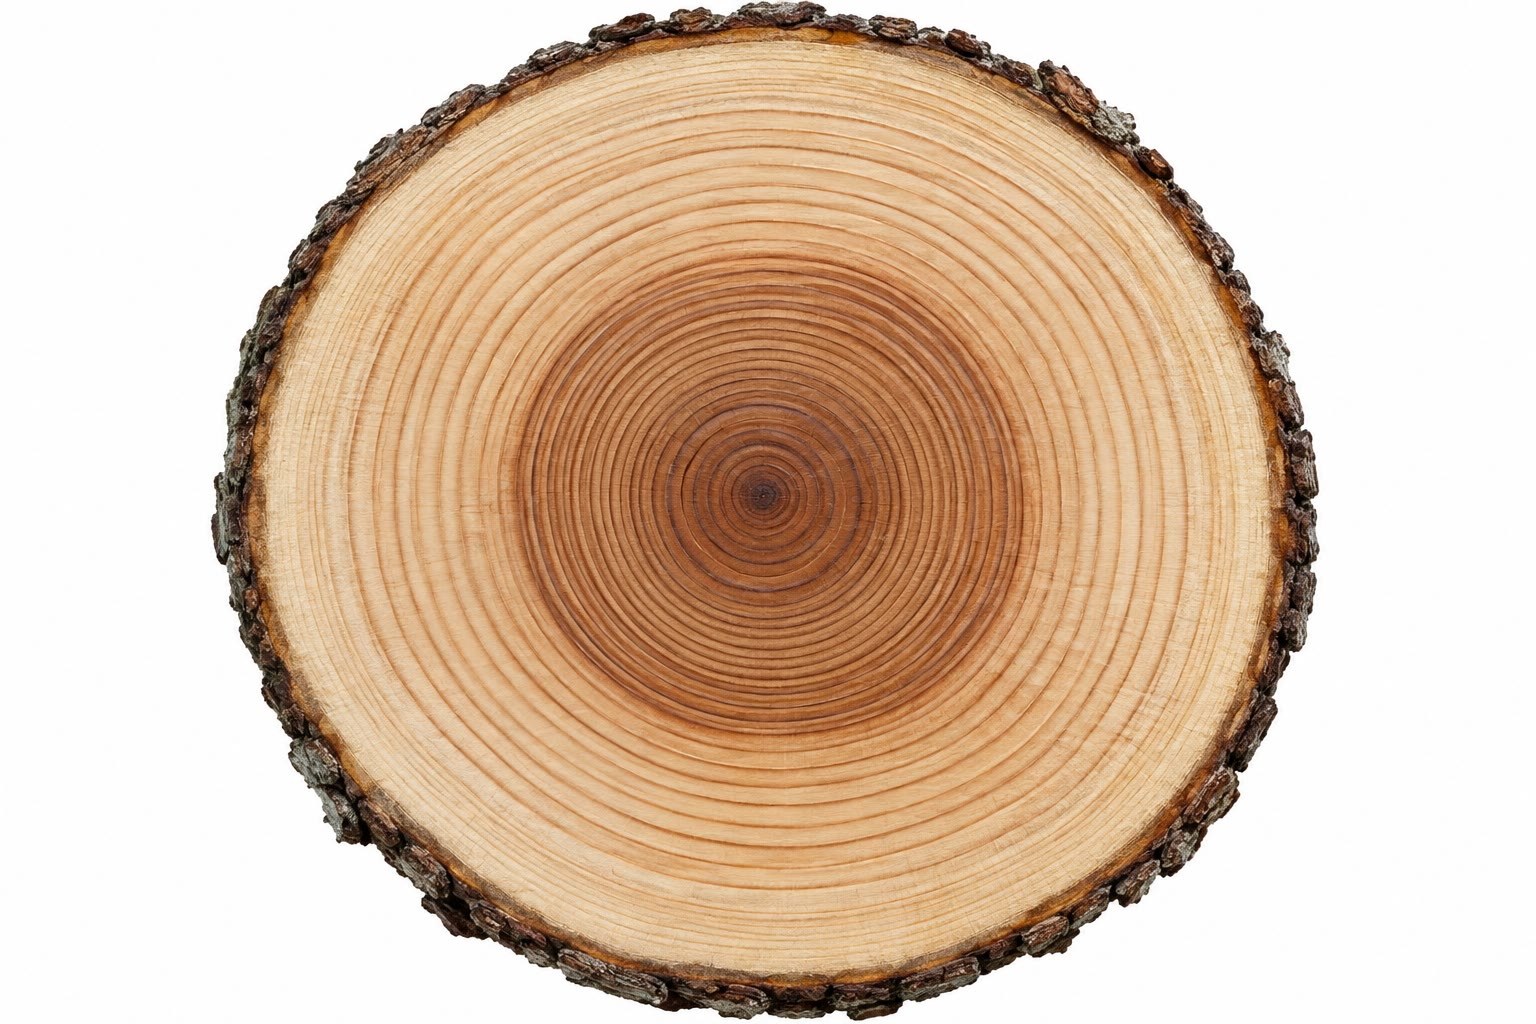
\includegraphics[width=0.5\linewidth]{images/book4/ai/b4-13-wood-rings.jpg}

{\small 松树树干横切面：\omterm{def:b2:plant-meristems:wood}{年轮}，每圈由浅色的
早材带和深色晚材带组成，其中较暗的为心材，
以及\omterm{def:b2:plant-meristems:wood}{树皮}。}
\end{omfigure}

\section{练习}

\begin{exercise}[$\star$]\label{exo:b2:plant-meristems:1}
定义\omterm{def:b2:plant-meristems:meristem}{分生组织}，并指出木本植物的四种\omterm{def:b2:plant-meristems:meristem}{分生组织}，
及各自产生的组织。
\end{exercise}

\begin{exercise}[$\star$]\label{exo:b2:plant-meristems:2}
自\omterm{prop:b2:plant-meristems:ram}{根冠}向上列出根尖各区，并说明
每个区中细胞发生的变化。侧根来自何处？
\end{exercise}

\begin{exercise}[$\star$]\label{exo:b2:plant-meristems:3}
叙述蒂曼–斯库格实验，说明其对照组及
结论。
\end{exercise}

\begin{exercise}[$\star$]\label{exo:b2:plant-meristems:4}
某树干切片显示 60 圈\omterm{def:b2:plant-meristems:wood}{年轮}，其中外层 15 圈为浅色，
求该树的树龄、边材的年龄，并说明树干的
哪一部分是活的。
\end{exercise}

\begin{exercise}[$\star\star$]\label{exo:b2:plant-meristems:5}
已知 $\phi = \qty{0.1}{h^{-1}.MPa^{-1}}$，$Y = \qty{0.3}{MPa}$，计算
在 $P = 0.4$、$0.6$ 及 \qty{0.8}{MPa} 时的相对生长速率，以及
各自对应的倍增时间。若干旱使 $P$ 降至 \qty{0.25}{MPa}，
则会出现什么情况？
\end{exercise}

\begin{exercise}[$\star\star$]\label{exo:b2:plant-meristems:6}
相继生成的叶片彼此相隔 \qty{137.5}{\degree}。
计算第 1 至第 8 片叶的角位置（模
\qty{360}{\degree}），并证明前八片叶中任意两片
之间的夹角都不小于 \qty{20}{\degree}。这对
植物有何意义？
\end{exercise}

\begin{exercise}[$\star\star$]\label{exo:b2:plant-meristems:7}
一棵高 \qty{12}{m} 的树，\omterm{def:b2:plant-meristems:wood}{年轮}每年增厚 \qty{3}{mm}。计算
树的半径为 \qty{5}{cm} 的那一年
与半径为 \qty{40}{cm} 的那一年所增加的\omterm{def:b2:plant-meristems:wood}{木材}，以及相应的碳含量（干密度
为 \qty{500}{kg/m^3}，其中一半为碳）。
\end{exercise}

\begin{exercise}[$\star\star$]\label{exo:b2:plant-meristems:8}
预测 \emph{clv3} \omterm{def:b2:genome-diversification:mutation}{突变}体、\emph{wus} \omterm{def:b2:genome-diversification:mutation}{突变}体和双\omterm{def:b2:genome-diversification:mutation}{突变}体的\omterm{def:b2:meiosis-heredity:vocabulary}{表型}，
并由双\omterm{def:b2:genome-diversification:mutation}{突变}体说明两个基因在
该调控回路中的先后顺序。
\end{exercise}

\begin{exercise}[$\star\star$]\label{exo:b2:plant-meristems:9}
\omterm{prop:b2:plant-meristems:apical}{生长素}以 \qty{1}{cm/h} 的速度运输，其在组织中的扩散系数为
\qty{1e-9}{m^2/s}。信号靠运输到达顶端以下 \qty{20}{cm} 处的
芽需要多长时间，靠扩散需要多长时间（
$t = x^2/2D$）？\omterm{prop:b2:plant-meristems:apical}{极性运输}对植物有何好处？
\end{exercise}

\begin{exercise}[$\star\star\star$]\label{exo:b2:plant-meristems:10}
玉米根每天生长 \qty{3}{cm}。\omterm{def:b2:plant-meristems:meristem}{分生组织}细胞
长 \qty{20}{\micro m}，成熟前伸长为原来的十倍；每列细胞
中约有 \num{100} 个正在分裂的细胞。每列\omterm{def:b2:plant-meristems:meristem}{分生组织}每天
须产生多少个细胞，由此可推出细胞周期的时长
为多少？
\end{exercise}

\begin{exercise}[$\star\star\star$]\label{exo:b2:plant-meristems:11}
20 世纪 60 年代的半矮秆小麦携带某些\omterm{def:b2:genome-diversification:mutation}{突变}，使植株
对赤霉素不敏感。试解释它们为何矮小，矮秆植株在大量施肥时为何
能产出更多籽粒，以及同一\omterm{def:b2:genome-diversification:mutation}{突变}若出现在野生植株中为何
会成为不利因素。
\end{exercise}

\begin{exercise}[$\star\star\star$]\label{exo:b2:plant-meristems:12}
“动物只建造一次；植物则终生都在建造自身。”试讨论
\omterm{def:b2:plant-meristems:meristem}{分生组织}生长对植物应对环境、承受损伤
以及存活数千年的能力所产生的影响，
并指出这一策略的一项代价。
\end{exercise}

\section{问题：数字中的一棵树}

\begin{problem}[{周末问题——追踪一棵幼树一年：
其顶端产生的叶，依洛克哈特定律的节间生长，
形成层沉积的木材及其耗费的碳，以及
芽对修剪的反应，最后归结为每年的叶数、
节间每小时的生长量以及全年的木材量}]
\label{pb:b2:plant-meristems:1}
一棵幼年椴树有 \num{200} 个正在生长的茎尖；每个顶端
在 \num{150} 天的生长季中，每 \num{3} 天起始一片叶，
相邻叶间隔 \qty{137.5}{\degree}。正在生长的节间
长 \qty{2}{cm}，其细胞的 $\phi = \qty{0.05}{h^{-1}.MPa^{-1}}$，$Y =
\qty{0.35}{MPa}$；膨压白天为 \qty{0.55}{MPa}，夜间为
\qty{0.75}{MPa}（白天和夜间各 \qty{12}{h}）。树干高
\qty{8}{m}，半径为 \qty{10}{cm}；\omterm{def:b2:plant-meristems:meristem}{形成层}每年
增加 \qty{5}{mm}；干\omterm{def:b2:plant-meristems:wood}{木材}密度为 \qty{500}{kg/m^3}，其中一半为碳。
树冠承载 \qty{80}{m^2} 的叶，
在 \num{150} 天内每平方米每天净固定 \qty{4}{g} 碳。

\medskip
\noindent\textbf{第一部分——叶。}
\begin{enumerate}
  \item 一个顶端在一个生长季中产生多少片叶？整棵
        树共产生多少片叶？
  \item 计算一根枝条上第 1 至第 5 片叶的角位置。
  \item 经过多少片叶之后，有一片叶会落在
        与第 1 片叶相差 \qty{10}{\degree} 以内的位置？（试取
        \qty{137.5}{\degree} 的倍数。）
  \item 黄金角对植物有何作用，
        这一角度由哪种激素的运输产生？
  \item 若每片叶的面积为 \qty{80}{cm^2}，则
        树在一个生长季中新建的叶面积是多少？与
        其仲夏时承载的 \qty{80}{m^2} 相比如何？
  \item 这棵树为落叶树。每年春季它重建的叶面积
        占其原有叶面积的比例是多少？最初几片叶所需的碳
        从何而来？
  \item \emph{clv3} \omterm{def:b2:genome-diversification:mutation}{突变}使每个顶端的大小增为三倍，
        则第 1 题和第 5 题的答案会有何变化，
        枝条又会呈现何种形态？
\end{enumerate}

\medskip
\noindent\textbf{第二部分——节间。}
\begin{enumerate}[resume]
  \item 计算白天和夜间的相对生长速率。
  \item 计算一个白天和一个夜间增加的长度，
        起始长度为 \qty{2}{cm}。
  \item 经过四个这样的昼夜后，节间长度为多少？
        （将生长视为复合增长，$L(t) = L_0 e^{rt}$，
        取平均速率。）
  \item 赤霉素处理使 $Y$ 降至 \qty{0.25}{MPa}。
        重新计算白天和夜间的速率。
  \item 干旱使白天和夜间的膨压均保持在 \qty{0.4}{MPa}，
        计算该速率，并说明渗透调节起何作用。
  \item 解释为何夜间生长量超过白天，
        尽管光合作用发生在白天。
\end{enumerate}

\medskip
\noindent\textbf{第三部分——\omterm{def:b2:plant-meristems:wood}{木材}。}
\begin{enumerate}[resume]
  \item 计算今年新增\omterm{def:b2:plant-meristems:wood}{木材}的体积及其干质量。
  \item 计算其中所含的碳。
  \item 计算整个生长季中树冠固定的碳。
  \item 树冠所固定的碳中，有多大比例进入了树干\omterm{def:b2:plant-meristems:wood}{木材}？
        另列举出三个其他的库。
  \item 二十年后，若\omterm{def:b2:plant-meristems:wood}{年轮}宽度保持不变，年\omterm{def:b2:plant-meristems:wood}{木材}增量将是多少？
        它为何会增大？
  \item 树干上有两个\omterm{def:b2:plant-meristems:wood}{年轮}，其宽度仅为相邻\omterm{def:b2:plant-meristems:wood}{年轮}的一半。
        试提出两种可能的原因，并说明树木年代学家
        如何将二者区分开来。
\end{enumerate}

\medskip
\noindent\textbf{第四部分——芽与修剪。}
\begin{enumerate}[resume]
  \item 园丁剪去每一个茎尖。预测
        一个月后腋芽的反应以及树的形态。
  \item 若在每个切口涂抹\omterm{prop:b2:plant-meristems:apical}{生长素}膏，这一反应会如何改变？
  \item 一道树篱每年修剪六次。试结合\omterm{prop:b2:plant-meristems:apical}{顶端优势}，
        解释它为何会变得浓密。
  \item 一棵被截成树桩的树会重新长出十二根枝条。
        这些枝条从何而来？植物为何能在失去全部枝条后存活，
        而动物失去头部却无法存活？
  \item 浇水后，来自根部的\omterm{prop:b2:plant-meristems:apical}{细胞分裂素}含量上升。
        预测其对芽萌发的影响。
  \item 陈述结果：每个顶端及每棵树在一个生长季中的叶数、
        节间白天和夜间的生长速率，以及当年的
        \omterm{def:b2:plant-meristems:wood}{木材}量与碳量。
\end{enumerate}
\end{problem}
